\section{有限差分}
有限差分是计算机求解微分方程的基本方法,这神方法的最佳特点就是它可以分析几乎
任何形态的对象、诸如大地地形或地质构造等。进行差分计算通常是一种简单的任务,其主
要问题是不稳定性。往往发生这样的现象,对一个合理的物理问题看来是合理的处理方法却
导致剧烈振荡和不收敛的计算结果。幸好,还有十分稀少的一些重要而又易于掌握的技巧可
以解决大多数不稳定性问题。

具有次要意义的一些问题是计算时间与精度问题。由于要付出更精细计算网格这样的高昂
代价方可改善精度,所以必须将计算时间与精度二者综合加以考虑。虽然选择以下几节所述方
法并非出于对猜度或计算效率的考虑,不过在这些领域内,这些方法确实是出色的。说实在的,
据我所知,某些方法完全不可能再改进了,而另一些方法改进的余地则可能很小。所谓“小”,
我的意思是指效率提高不超过五倍的改进。这样的改进很少是由于研究或试验工作的结果。
然而,鉴于它对生产工作具有重要性,进一步阅读远超出以下几节内容的文献还是很必要的。

\subsection{透镜方程}
各种波场外推算子均可分为两部分:较复杂的部分称为绕射或偏移部分,而较简单的部
分则称作透镜部分。透镜方程引入了一个作为$x$之函数的时移,由于它正像一个光学薄透镜
在光线沿轴向投射(垂直投射)时那样起作用,故而获得透镜方程这种名称。在绕射部分
中,以某种方式隐含着对非垂直入射和透镜厚度的校正.透镜方程存在有解析解,即$\exp[i\omega t_0(x)]$
。运算时,最好是利用这种解析解而不是利用某种差分解,因为解析解没有因采用近
似计算而引起的误差。在讨论有限差分的一章中之所以会提到透镜方程,其仅有的原因完全是
由于伴随的绕射方程必须与透镜方程一起向前推进计算,所以解析解要沿很小的步长推进。

\subsection{一次导数与显式方法}

速率为10\%的通货膨胀率$q$可用下述差分方程描述
\begin{subequations}
\begin{equation}
q_{t+1}-q_t=0.10q_t
\label{eq:2.2.1a}
\end{equation}
\begin{equation}
(1.0)q_{t+1}+(-1.1)q_t=0
\label{eq:2.2.1b}
\end{equation}
\label{eq:2.2.1}
\end{subequations}
这类一维计算可用差分系数表和数据表重新加以表示,就这一点而论,它对如何组织二维偏
微分方程的计算提供了一种范例。设有下列系数表与数据表
\begin{figure}[H]
\centering
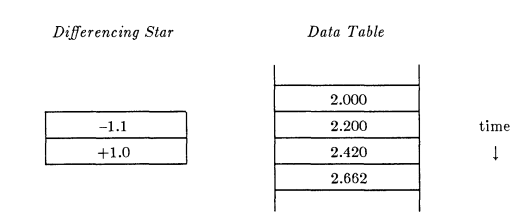
\includegraphics[width=0.5\textwidth]{new/datatable}
\caption[datatable]{差分系数表和数据表}
\label{fig:new/datatable}
\end{figure}
由于数据表中的数据满足差分方程\ref{eq:2.2.1},可将差分系数表置于数据表顶部的任何地
方。将系数表中的数乘以它下面的表中的那些数,所得互乘结果之和将为零。另一方面,如
果数据表中除一个数(初始条件)之外,所有的数都没有,则可沿时间増大方向滑动该系数
表。取互乘之和并令差分方程成立,一次计算出一个数,每一步都可解出未知数据值,从而
可将数据表中所有其余的数部填满。

当数值系数0.10周一个复数代替时,利用同一套差分系数表就要稍为繁琐一些。这种情
形下,计算结果既表现出有振荡现象,又表现出有增大和阻尼衰减的现象。

\subsection{一次导数与隐式方法}
试以数值方法求解下述方程:
\begin{equation}
\frac{dq}{dt}=2rq
\label{eq:2.2.3}
\end{equation}
注意,在通货膨胀方程\ref{eq:2.2.1}中是$2r=.l$,那种方程是一种近似式,但是现在要注意,在
通货膨胀方程中的表达式$dq/dt$是位于时间$t+1/2$,而表达式$q$本身则位于时间$t$。没有理由
不把式\ref{eq:2.2.3}右端的$q$在时间$t$上用时间$t+1$来加以平均,因而可将整个方程均置于时间
$t+1/2$。具体说,式\ref{eq:2.2.3}的中心差分近似为
\begin{subequations}
\begin{equation}
q_{t+1}-q_t=2r\Delta t\frac{q_{t+1}+q_t}{2}
\label{eq:2.2.4a}
\end{equation}
令$\alpha=r\Delta t$,上式变为
\begin{equation}
(1-\alpha)q_{t+1}-(1+\alpha)q_t=0
\label{eq:2.2.4b}
\end{equation}
\label{eq:2.2.4}
\end{subequations}
\begin{figure}[H]
\centering
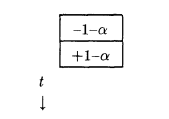
\includegraphics[width=0.25\textwidth]{new/difftable}
\caption[difftable]{差分系数表}
\label{fig:new/difftable}
\end{figure}
在固定步长的情形下,这种系数表得出的微分方程\ref{eq:2.2.3}的解比前述由通货膨胀系数表得出的解更为精确。

\subsection{显式热流方程}
热扩散系由热流方程控制.这种方程是地震偏移方法的一个原型,15°偏移方程与该方
程形式相同,只不过热传导常数是虚数而已(偏移方程实际是Schroedinger方程,该方程
描述原子粒子扩散几率)。取$\sigma$为常数,得热流方程
\begin{equation}
\frac{\partial q}{\partial t}=\frac{\sigma}{c}\frac{\partial^2 q}{\partial x^2}
\label{eq:2.2.5}
\end{equation}
在计算机上实现式\ref{eq:2.2.5}的计算需对各偏微分作某种差分近似。最明显不过(但并非
唯一的)的办法就是采用初等微积分教程中关于微分的基本定义,就时间导数而言,这就
是
\begin{subequations}
\begin{equation}
\frac{\partial q}{\partial t}\approx \frac{q(t+\Delta t)-q(t)}{\Delta t}
\label{eq:2.2.6a}
\end{equation}
利用下标使式\ref{eq:2.2.6a}形式紧凑是很方便的
\begin{equation}
\frac{\partial q}{\partial t}\approx \frac{q_{t+1}-q_t}{\Delta t}
\label{eq:2.2.6b}
\end{equation}
\end{subequations}
在这种符号表示中,$t+\Delta t$简记为$t+1$,对于更为复杂的方程有其方便之处。取两次一阶导
数可得到二阶导数公式,由此得出$q_{t+2}-2q_{t+1}+q_t$;通常都进行时移,将该公式处理成更
为对称的形式$q_{t+1}-2q_t+q_{t-1}$。当$\Delta t$趋于零时,这两种形式是等价的,但是在$\Delta t$不为零
时,则更为对称时安排形式将更为精确。利用上标描述与$x$有关的函数,得出二阶空间导数
的有限差分近似:
\begin{equation}
\frac{\partial^2 q}{\partial x^2}\approx \frac{q^{x+1}-2q^x+q^{x-1}}{\Delta x^2}
\label{eq:2.2.7}
\end{equation}
将\ref{eq:2.2.6b}与\ref{eq:2.2.7}代入热流方程,并用符号$=$表示$\approx$,得
\begin{equation}
\frac{q_{t+1}-q_t}{\Delta t}=\frac{\sigma}{c}\frac{q_t^{x+1}-2q_t^x+q_t^{x-1}}{\Delta x^2}
\label{eq:2.2.8}
\end{equation}
令$a=\sigma \Delta t/(c\Delta x^2)$时,式\ref{eq:2.2.8}可重写为
\begin{equation}
q_{t+1}-q_t-a(q_t^{x+1}-2q_t^x+q_t^{x-1})=0
\label{eq:2.2.9}
\end{equation}
几何上,可将式\ref{eq:2.2.9}解释为$(x,t)$平面中的一种十字形系数表的计算结果,如
图\ref{fig:new/fig2-2-1}所示。在数据表内移动该十字形系数表,你会注意到,它可一次仅将一个数定位于
数据表内之未知元素位置上(即在1所指示的位置上),这就使得能从数据表顶部开始依次
计算下一行.照这样作下去,你就是在用有限差分方法求解偏微分方程。关于初始条件和边
界条件还存在其他可能的安排,诸如零斜率边界条件等。下面是一个计算机程序和验算的例
子。
\begin{figure}[H]
\centering
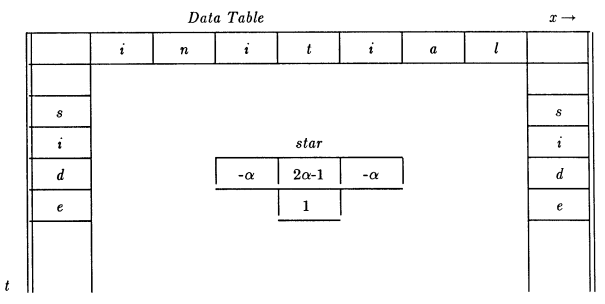
\includegraphics[width=0.95\textwidth]{new/fig2-2-1}
\caption[fig2-2-1]{一维热流方程的十字形差分系数表与数据表}
\label{fig:new/fig2-2-1}
\end{figure}
\begin{minted}{Fortran}
# Explicit heat-flow equation 
real q(12),qp(12) 
nx= 12

do ia== 1,2 { # stable and unstable cases

alpha = ia* . 3333 ; write(6, '(/"alpha=",f4.2)')alpha 

do ix= 1,6; q(ix) = 0. # Initial temperature step
do ix=7,12; q(ix) = l. 
do it= 1,6 {

write(6 , '(20f5.2)') (q(ix),ix=1,nx) 
do ix=2,nx-l
qp(ix) = q(ix) + alpha* (q(ix-1)-2. * q(ix)+q(ix+1)) 
qp(1) = qp(2);
qp(nx)=qp(nx- 1) 
do ix = 1 ,nx
q(ix) = qp(ix)
}
}
stop;end

alpha=.33
0.00 0.00 0.00 0.00 0.00 0.00 1.00 1.00 1.00 1.00 1.00 1.00 
0.00 0.00 0.00 0.00 0.00 0.33 0.67 1.00 1.00 1.00 1.00 1.00
0.00 0.00 0.00 0.00 0.11 0.33 0.67 0.89 1.00 1.00 1.00 1.00
0.00 0.00 0.00 0.04 0.15 0.37 0.63 0.85 0.96 1.00 1.00 1.00
0.00 0.00 0.01 0.06 0.19 0.38 0.62 0.81 0.94 0.99 1.00 1.00
0.00 0.00 0.02 0.09 0.21 0.40 0.60 0.79 0.91 0.99 1.00 1.00

alpha=.67
0.00 0.00 0.00 0.00 0.00 0.00 1.00 1.00 1.00 1.00 1.00 1.00 
0.00 0.00 0.00 0.00 0.00 0.67 0.33 1.00 1.00 1.00 1.00 1.00
0.00 0.00 0.00 0.00 0.44 0.00 1.00 0.56 1.00 1.00 1.00 1.00
0.00 0.00 0.00 0.30 -.15 0.96 0.04 1.15 0.70 1.00 1.00 1.00
0.00 0.00 0.20 -.20 0.89 -.39 1.39 0.11 1.20 0.80 1.00 1.00
0.13 0.13 -.20 0.79 -.69 1.65 -.65 1.69 0.21 1.20 0.87 0.87
\end{minted}
\subsection{鞋跃式方法}
